\documentclass[12pt,a4paper]{article}
\usepackage[utf8]{inputenc}
\usepackage[margin=0.5in]{geometry}
\usepackage{amsmath}
\usepackage{amsfonts}
\usepackage{amssymb}
\usepackage{graphicx}
\author{Keith Drew \& Tyler Jaszkowiak}
\title{Diagram Assembly Document}
\begin{document}
\maketitle
\begin{itemize}
\item Board: The game board, this holds nearly all visual information about the game and state. The class holds random event flags, which will become more specific, that indicate global events.
\item Province: A province is a group of hexes that are related by controlling faction. Essentially like the United States of Hexes. 
\item Hex: A discrete location on the board. Hexes are represented by a unique ID, terrain, and a stack of units that can be empty.
\item Stack: A collection of units and characters, bound by the rules of the game. Ie, 0 or more characters, and 0-2 units. Also, special considerations for movement phase, flying units, and monsters.
\item Special Hex: The special hex can be any of the residential hexes (city/capital/town/castle), or it can be one of the several unique hex types, such as a teleport hex or vortex hex, or the terrifying Bottomless Plungehole. 
\item Vortex: A vortex is a moveable unit, from the system's point of view. A character can control vortices under certain conditions. Otherwise movement, creation, and destruction of vortices is automated.
\end{itemize}
\begin{verbatim}
@startuml
title Keith Drew \& Tyler Jaszkowiak Class Diagrams\nMap Related
hide circle

class Board #529292 {
      List Provinces
      RandomEventFlags (misc)
      int gameTurn
      int gameTurnLimit
}

class Province #529292 {
      String provinceName
      String GetName()
      List Allies
      HexContainer Hexes
}
note right of Province #red
     Provinces may only have one Capitol
     type hex in it's composition.
end note 

class Hex #529292 {
      int hexID
      double moveCost
      double terrainID
      UnitStack units
      double GetTerrainID()
      int GetHexID()
      void ChangeTerrainType()
}
class Stack #529292 {
      List Units
      List Characters
      Stack SelectSubStack()
      void RemoveExcessUnits()
}
class SpecialHex #529292 {
      String name
      String hexType
      String GetHexType()
      String GetName()
}
class ResidentialHex #529292 {
      int leadershipRating
      double initialDefenseRating
      double defenseRating
      double GetDefenseRating()
}
class BottomlessPlungeHole #529292 {
      void DestroyStack()
}
note left of BottomlessPlungeHole #red
     If any units move here, 
     they are destroyed.
end note 

class VortexHex #529292 {
      void SpawnVortex()
}
class TeleportHex #529292 {
      void TeleportUnits()
      int teleportID
}
class Vortex #529292 {
      double moveableUnitID
      void RandomMovement()
      void DamageUnits()
      void Move()
}

Board *-right- "22" Province : Provinces build\nboard 
Province *-down- "1..*" Hex : Hexes build\nProvinces
Hex <|-down- SpecialHex : Extends
Vortex .up. VortexHex : Spawns
note right on link #red
     This is where vortices come
     from, other than spells.
end note  

TeleportHex --up|> SpecialHex : Extends
VortexHex --left|> SpecialHex : Extends
BottomlessPlungeHole --right|> SpecialHex : Extends
ResidentialHex --up|> SpecialHex : Extends
Stack -lefto Hex : Aggregation
@enduml
\end{verbatim}

\pagebreak
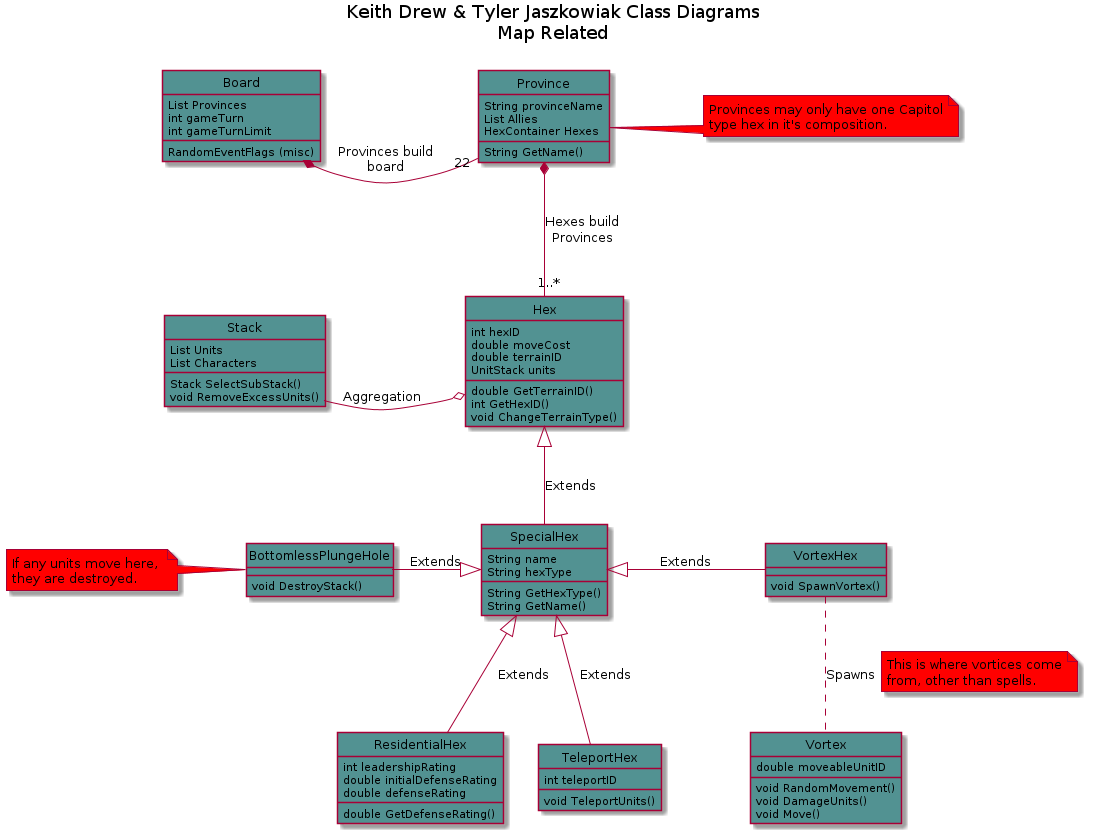
\includegraphics[width=\textwidth]{classD}
\end{document}